\chapter[Description]{Description of program}
\label{chap:description}

\section{Program structure}
The developed application is divided into three modules as seen in figure \ref{fig:program_structure}

\begin{figure}[!h]
  \centering
  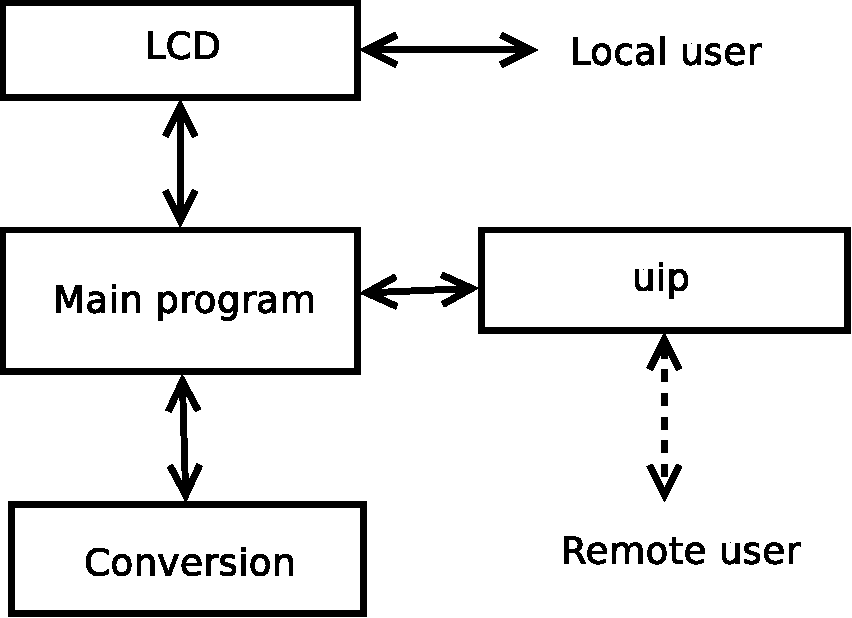
\includegraphics[width=0.5\textwidth]{figs/program_structure.pdf}
  \caption{The overall program structure}
  \label{fig:program_structure}
\end{figure}

The conversion part is responsible for most of the ADC, DAC, GPIO and interrupt handling parts of the program. The LCD is taking care of the physical user interface, both touchscreen and displaying values on the screen. The uip is accepting remote connections and serving data to remote clients.\\\\
The program runs roughly this sequence depicted in figure \ref{fig:program_sequence}

\begin{figure}[!h]
  \centering
  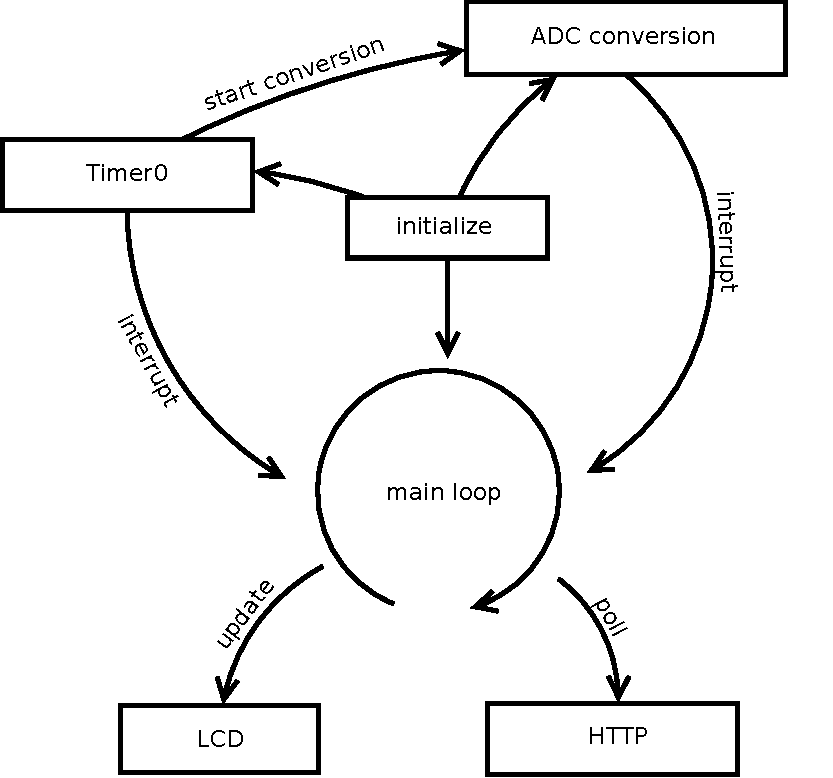
\includegraphics[width=0.6\textwidth]{figs/program_sequence.pdf}
  \caption{The overall program sequence}
  \label{fig:program_sequence}
\end{figure}

The first thing done is the initialization. This obviously only run once. It gets the interrupts up and running and configures the appropriate GPIO pins. When done, it enters the main loop, where the application remains for remainder of run-time, while not processing interrupts.\\
The Timer0 runs at a predefined frequency, and takes care of starting the ADC conversion process, reading the touchscreen coordinates, detect zero-crossings, do http timer ticks and controlling relays.\\\\
The ADC interrupt detects touches to the screen and stores the data from the measurements, does filtering and accumulates the squared values (integrates), used to calculate the corresponding RMS values.\\\\
When not doing interrupts the main loop updates the screen, checks if a user has touched the screen and moves the cursor accordingly.\\
It also does periodic checks on the IP stack, sending and receiving packets at a reasonably stable frequency. This is done via the HTTP server.
\subsubsection{Debugging the timing}
Throughout our development process we had to verify that no single interrupt took so long time to execute that the next interrupt was delayed.\\\\
We thought of three possible ways to ensure this.\\
One method is to start another timer at the start of the interrupt routine, and stop it again at the end. We would now have the time the interrupt routine took.\\
Another method would be to clear the timer interrupt flag at the start of the interrupt routine and check the register at end of the routine. If it is high again - then our interrupt routine takes too long.\\
The third method is to output a logical high signal to the DAC at the start of the interrupt routine, and then low again at the end of the routine. This was the method we used.

\section{Measurements and control}
\subsection{GPIO}
We are using a number of GPIO's for various purposes. For example we are using P[1]\_18 and P[1]\_13 for LED's, P[0]\_11 and P[0]\_19 for controlling the relays. Other GPIO's are used in the touchscreen handling.

\subsubsection{ADC}
To get the maximum number of samples per second, we use burst mode (illustrated in figure \ref{fig:burst_mode}). As this enables us to free up some cpu time and make the conversion faster.
\begin{figure}[!h]
  \centering
  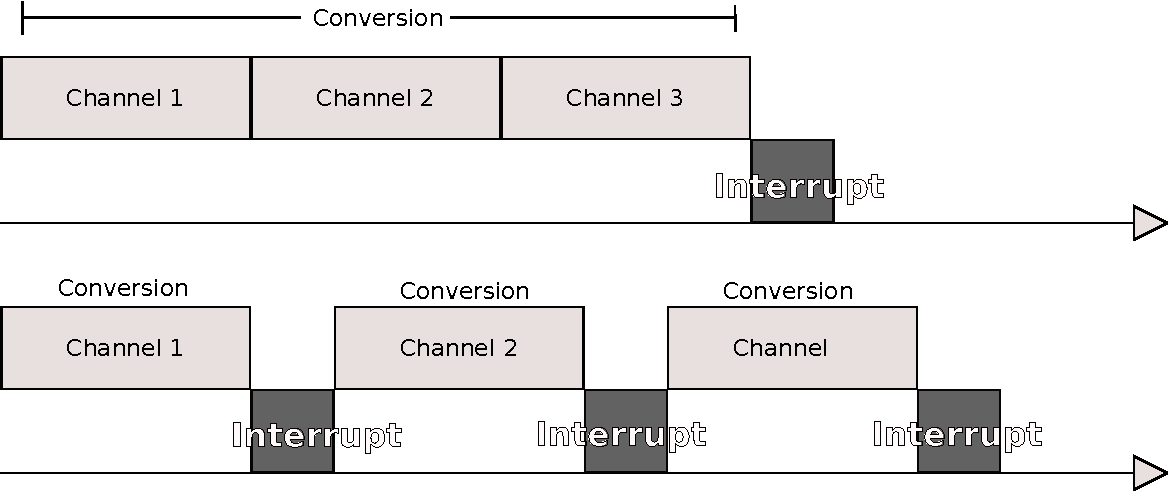
\includegraphics[width=0.85\textwidth]{figs/burst_mode.pdf}
  \caption{Illustration of the principle behind burst mode}
  \label{fig:burst_mode}
\end{figure}
The burst is started by entering the Timer0 interrupt handler, and runs simultaneously with our main loop and Timer0 handler. This is of course due to the fact that the conversion is done in hardware and does not need the processor for calculations.

\subsection{Measurement algorithms and their implementation}
The values measured with the micro-controller (ADC) are:
\begin{itemize}
\item Grid frequency
\item Grid voltage
\item Grid current
\item LCD voltage (checking if, and if so, where LCD screen has been touched)
\end{itemize}

\subsubsection{Voltage and Current measurements}
The voltage from the grid is passed through a circuit that lowers it's value to 0...3.3V range, before it can be processed by the micro-controller. The same thing is done with the current - it is converted to a voltage signal of the same scope. Both signals are scaled afterwards so the output of calculations is in grid values. Two different approaches were used for each of them.

\paragraph{Voltage scaling}
Firs the RMS and offset values of the grid voltage has been measured. The results were:\\\\ 
\[ V_{RMS}=236V \] 
\[ V_{Offset} \approx 0V\]\\
then assuming that the offset value corresponding to 0 V is exactly half of the measurement range of the ADC we set this to 512. After subtracting this value 
from the raw data we get the raw data RMS value. This value together with the measured RMS voltage can be used to scale the raw data to physical values in 
volts. The raw data RMS value is 341 which means that the scaling factor for RMS voltage is
\[ V_scalefactor= 236V/341=0,692082\]

\paragraph{Current scaling}
A bit different approach have been used while calculating the scaling ratio in the case of the grid's current. Here we've assumed that the current converting 
circuit is very precise and that the output values are exactly 0....3.3V. Thus we can expect that the quantization level corresponding to 0A is equal to 512. 
Because we can not really measure the actual current in the system we assume that the system uses the full measuring range this means that the RMS current 
signal in raw data values should be 
\[ Iraw_{RMS}=512/\sqrt(2)=362\]
The specified maximum RMS current is 1A which gives us a current scaling factor of  
\[ V_scalefactor= 1/362=0,00276243\]

\subsubsection{Frequency measurement}
The frequency measurement is done by calculating the length of the period of a given signal. It is done by calculating the number of samples between the points at which the signal is crossing an arbitrarily defined zero line with an assumed direction (rising edge or falling edge) and comparing it (number of samples) with the sampling frequency.\\
In order to detect zero-crossing two succeeding samples have to be remembered by the system. If the previous sample was below the zero-level and the current one is above, than the system marks this time as a rising edge zero-crossing and starts to count the samples until the next one.\\
Due to significant disturbances a low pass filter has to be used, in order to smoothen out the data. Without it detecting false zero-crossings would be very common, which in turn would render the method completely useless.\\
The low-pass filter is used only for this particular purpose, though. All the other calculations, like voltage RMS value, power etc. are performed on raw data. That is due to the fact that the filters output differ significantly from its input (the amplitude is attenuated and the signal is shifted in phase). On the other hand filters, by definition, never change frequency, which make them useful in this particular case. This is shown on the Figure ~\ref{fig:filter}

\begin{figure}[!h]
  \centering
  \subfloat[Cut-off at 100Hz]{\label{fig:100@10}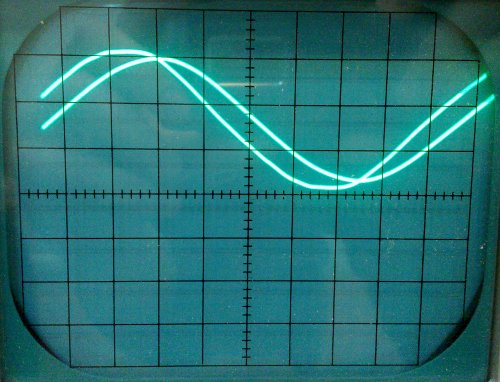
\includegraphics[width=0.3\textwidth]{img/used/100Hz@10kHz_small.png}}                
  \subfloat[Cut-off at 50Hz]{\label{fig:50@10}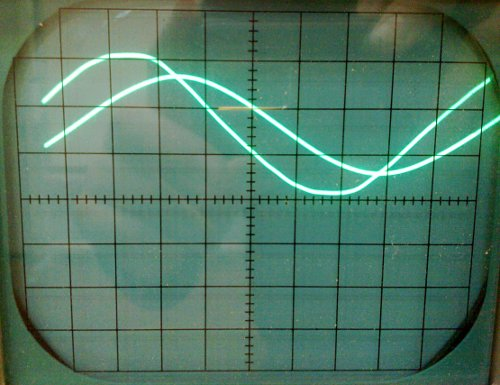
\includegraphics[width=0.3\textwidth]{img/used/50Hz@10kHz_small.png}}
  \subfloat[Cut-off at 10Hz]{\label{fig:10@10}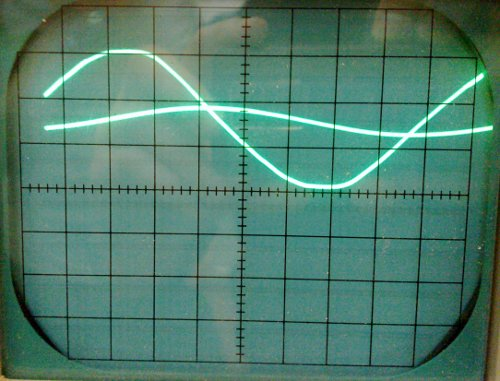
\includegraphics[width=0.3\textwidth]{img/used/10Hz@10kHz_small.png}}
  \caption{Input and output signals of a low-pass filter at a sampling frequency of 10kHz for three different cut-off frequencies.}
  \label{fig:filter}
\end{figure}


\subsubsection{LCD measurements}
The LCD measurements are conducted to check if the touch screen has been touched and if yes, where exactly did it happen. The possition of the touch is determined by measuring the voltage on the LCD's outputs. Measurement of the X and Y coordinates aren't done simultanously. If we want to measure the X coordinate the ADC and the pins have to be set to a certain state. In order to meassure the Y coordinate those set up options have to be different. This is due to the way that the measurements are conducted. The electrical setup of the LCD screen is depicted on Figure \ref{fig:LCD_screen_measurement}.

\begin{figure}
  \centering
  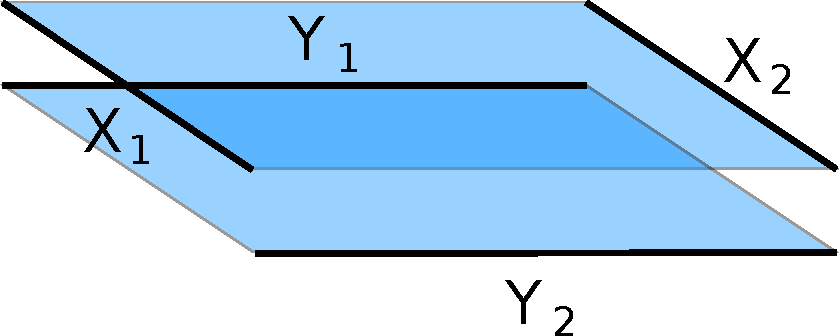
\includegraphics[width=0.75\textwidth]{img/used/adc_layers.pdf}               
  \caption{Simplified overview of a two layer LCD electrical setup.}
  \label{fig:LCD_screen_measurement}
\end{figure}

In order to measure the X coordinate of the touched place on the LCD screen a potential gradient has to be applied to the bars represented as X1 and X2 on Figure \ref{fig:LCD_screen_measurement}. The actual X coordinate is determined by measuring the voltage on the Y layer wich changes with the distance, from one of the X bars, at witch the touch accured. Applying a gradient in an opposite direction would cause the measurement to be giving position references with regards to the other side of LCD (X coordinates would measured from right to left instead of doing it in the left-to-right fashion). \\
Measuring Y coordinates requires seting up ADC and GPIO pins in reverse manner. Since every LCD output channel is hardwired to a different port and we need to change the GPIO configuration each time we want to reset ADC for measuring different coordinate, every coordinate is meassured only every second ADC action. The overview of connections needed for every ADC conversion cyckle is shown in the below table:

\begin{table}[!h]\caption{Simplified overview of a two layer LCD electrical setup.}\begin{tabular}{|l|l|l|l|l|}\hline & X normal & X reverse & Y normal & Y reverse \\ \hline $X_{1}$ (pin 24) & set to high & set to low & ADC input & ADC input \\ \hline $X_{2}$ (pin 22) & set to low & set to high & disabled & disabled\\ \hline $Y_{1}$ (pin 23) & ADC input & ADC input & set to high & set to low \\ \hline $Y_{2}$ (pin 21) & disabled & disabled & set to low & set to high \\ \hline\end{tabular}\label{table:LCD_screen_measurement} \end{table} 



\section{User interface}
The user interface's layout is presented below:\\
\begin{figure}[!h]
  \centering
  \subfloat[Main screen]{\label{fig:main_scr}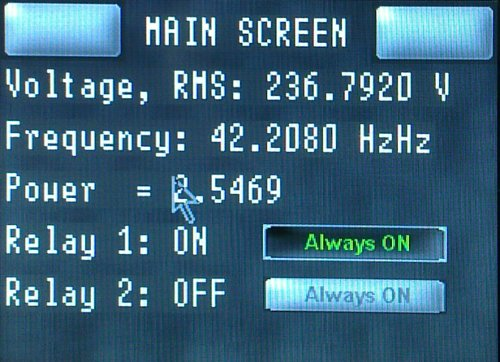
\includegraphics[width=0.3\textwidth]{img/main_menu_small.jpg}}       \subfloat[Config screen]{\label{fig:config_scr}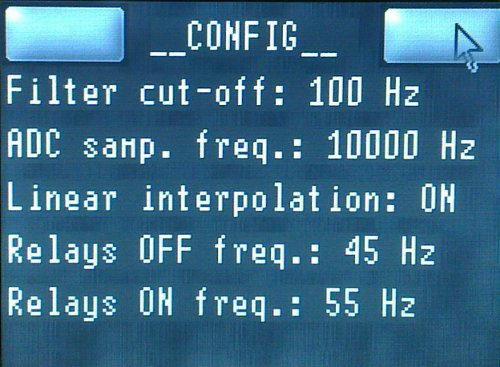
\includegraphics[width=0.3\textwidth]{img/config_small.jpg}}
  \subfloat[Test screen]{\label{fig:test_scr}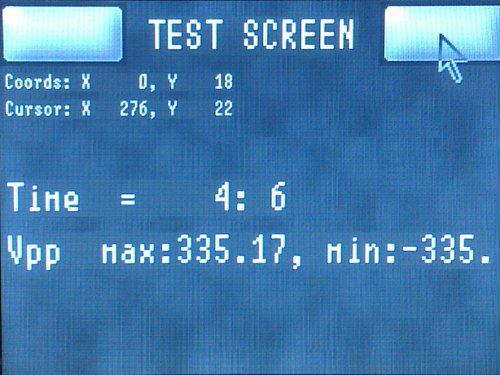
\includegraphics[width=0.3\textwidth]{img/test_screen_screen.jpg}}
  \caption{Screenshots of the graphical user interface parts}
  \label{fig:filter}
\end{figure}
It is build out of three different screens:
\begin{itemize}
\item Main screen
\item Config screen
\item Test screen
\end{itemize}
There is a panel's name label at the top of each screen. There are also two buttons on it's both sides. They allow the user to switch between screens in a ring fashion (if one button is pressed continuously, then the screens repeat their selves).\\

\subsection{Main screen}
The main screen is the default panel presented on the LCD. It shows the values of:
\begin{itemize}
\item $ Voltage_{RMS} $
\item Frequency
\item Power
\item State of relay 1
\item State of relay 2
\end{itemize}
\subsubsection{LCD measurements}
The LCD measurements are conducted to check if the touch screen has been touched and if yes, where exactly did it happen. The possition of the touch is determined by measuring the voltage on the LCD's outputs. Measurement of the X and Y coordinates aren't done simultanously. If we want to measure the X coordinate the ADC and the pins have to be set to a certain state. In order to meassure the Y coordinate those set up options have to be different. This is due to the way that the measurements are conducted. The electrical setup of the LCD screen is depicted on Figure \ref{fig:LCD_screen_measurement}

Apart from the above there are two bistable buttons, next to the information on the relay status. If they are on the system forces the relays to be switched on at all times. If not, the relays will be automatically  switched off if the grid frequency will drop below a certain level.

\subsection{Config screen}
This panel may depict some of the information on the configuration of the system [\emph{IMPLEMENT IN THE uC}]:
\begin{itemize}
\item The cut-off frequency of the low-pass filter
\item Sampling frequency
\item ADC conversion mode
\item Usages of the linearization function
\item Relay switch off frequency
\item Relay switch on frequency
\end{itemize}

\subsection{Test screen}
This panel may be used during the updating/debugging of the programme for displaying certain variables. Thanks to a special function ({\textit{enable\_line\_of\_text()}) only two simple lines of code are required to display a given text line in a specified position on the screen, which makes checking how certain variables change in the real time, fairly easy.

\section{Communication}
The communication part of the program is done by reusing the uip network stack. The built-in http server has the ability to both serve files and do some basic server-side scripting. \\
We plan on refactoring the server, making able to serve xml and xsl\footnote{XML Stylesheet} (with the right content-type). Xsl will enable us to generate a single xml file and then transform it for the user to view via a browser. The xml document will be treated as a regular html page, making the transformation transparent for the user. \\
The really nice thing about xsl is that we only need one source of information for both the user interface (webpage) and for automatically downloading done by programs interested in only the data. The programs will disregard the xml stylesheet and only fetch the data, minimizing overhead.
\subsection{Implementation}
The first step in getting the webserver working as we intended was getting the stand-alone server accepting xml files. This was relatively easy, and so was getting the server to generate content dynamically. This was mostly done by copy-pasting, and the code is included.\\
One thing that did baffle us though, was the fact that the uIP http server strings was written as arrays of bytes. Very unreadable and pointless, as a string or a char array would been just as good.\\\\
Our next step was getting the generic server merged into our main project. The big challenge was that the uip server used a global timer, and not just any timer - the same timer we already used i our main project.\\
The migration was again done in two steps. First step was moving the httpd timer from timer0 to timer1, and check if that worked. Next step was merging the code of the two timers into one, and get the timing right. The change from timer0 to timer1 resulted in a very slow, but working, webserver.\\\\
The problem in merging the two timers was due to the fact that they ran at two different frequencies. One at 20MHz and another at 100Hz. As these was both defined in our config.h as respectively TIMER0\_TICK\_PER\_SEC and HTTPD\_TICK\_PER\_SEC we figured we needed to add a counter and do the following:
\begin{equation}
  counter \% \frac{TIMER0\_TICK\_PER\_SEC}{HTTPD\_TICK\_PER\_SEC} = 0
\end{equation}
The \% is the modulus operation. Upon true, the counter should reset and the http tick should increment. This implementation should make the http server insensible to changes in the timer0 frequency.\\\\
The webpage itself refreshes every 5 seconds by asking the browser to do a delayed redirect to the same page.\\\\
Upon studying our code more closely, we discovered our slowdown was caused by the LCD doing refresh every free cputime it could get its dirty hands on. After getting the refresh down to 5Hz the server performance improved significantly. Later on in the coding process the webserver suffered another slowdown, which we have not been able to fix yet.

\subsubsection{Historical values}
Although not implemented, due to different focus, we have spent some time considering a possible implementation.\\
At first glance the buffer could be implemented using a linked list - but due to the fact that we do not have at memory manager we would at some point run out of free memory to store these these historical values. So, we could use a fixed size array of int pointers, and a pointer to the last element inserted. Then it should be possible to run through the array ``array-size'' number of times, starting from ``last\_inserted'' and break if we encounter a null pointer.\\
The historical values should be displayed on a graph generated as an svg image, using JQuery to reload the values without reloading the page.

\section{Chapter Summary}
\label{sec:SummaryDescription}
\subsection{Communication}
The finished result can be viewed by accessing the ip (typically 192.168.0.100) and requesting the data.xml document. When doing this from a browser the transformation works like a charm and gives us a graphical representation of our values. The server is still slow when we enable the LCD and touchscreen, but this should just a matter of optimizing the code that handles these.\\
The browser refresh is, agreed, a bit quick n' dirty, but also works as intended. The xsl and xml files is with the other files in the uip/http-fs folder.\\
For communication via TCP/IP on an intelligent power grid, we do not think that xml+http should be the way to go. The overhead would be too big in comparison to a binary protocol.
